\chapter{Evaluation} \label{chap:evaluation}

This chapter presents the results of the performance evaluation of the 
DADT/LN prototype running on real-world sensor nodes (Sun SPOTs). 

\section{Setting}

% Unless you already explained it somewhere else (and yet a reference to this
% "somewhere else" must be put in this chapter), the reader has very
%little information as to what your test application is doing. You need to give
%more details, say exactly what the application is supposed to accomplish and
%how.

The sample distributed application used for evaluation of the DADT/LN prototype 
implements an example WSN application where several sensor devices are deployed
in the environment and able to provide reports about some physical
phenomena, e.g. temperature. A monitoring station may access
particular sensor devices in WSN to aggregate their sensor readings, e.g. to
calculate average value, or reset sensors in case of problems.

The sample distributed application initially consists of the following files:
\begin{itemize}
  \item \emph{Sensor.java}, which defines the functionality of the device
  that provides sensing ability.
  \item \emph{SensorNode.dadt}, which defines the sensors and/or actuators available on the sensor
  device as abstract ADT instances, and binds them to the ``DSensor''  DADT type.
  \item \emph{ClientNode.dadt}, which is run by monitoring station
  in order to perform the distributed operation requests; the scope
  of the distributed operation is also declared here.
  \item \emph{DSensor.dadt}, which declares the list of available
  distributed operations, actions and properties.
\end{itemize}

As described in Section \ref{sec:PrototypeDesign}, the dadt files are translated
by DADT preprocessor into conventional java application. This
results into creation of additional java files, each of which represents DADT
Property and DADT Action classes (see Section \ref{subsec:DADTsConcepts}) that
were declared by application developer in \emph{DSensor.dadt} file. 

These files are named according the following naming scheme:
``DSensorXXXproperty'' or ``DSensorYYYaction'', where \emph{XXX} is a name of the
DADT Property and \emph{YYY} is a name of the DADT Action respectively. 

The functionality of the sample application is provided by the objects
of the runtime library of the DADT/LN prototype \ref{ADDREF}.  

The code of the distributed application is coupled with the
compiled runtime library to create 2 jar-files representing distributed
applications, namely the SensorNode and ClientNode applications, which were
deployed on the Sun SPOT devices.

6 Sun SPOT devices that form a simple WSN were used as a testbed for performing
their evaluation. Each of the Sun SPOT devices ran one of the LN/DADT prototype
distributed applications (ClientNode or SensorNode) application, as can be seen
in Figure \ref{Fig:EvaluationConfig}.

\begin{figure}
\centering
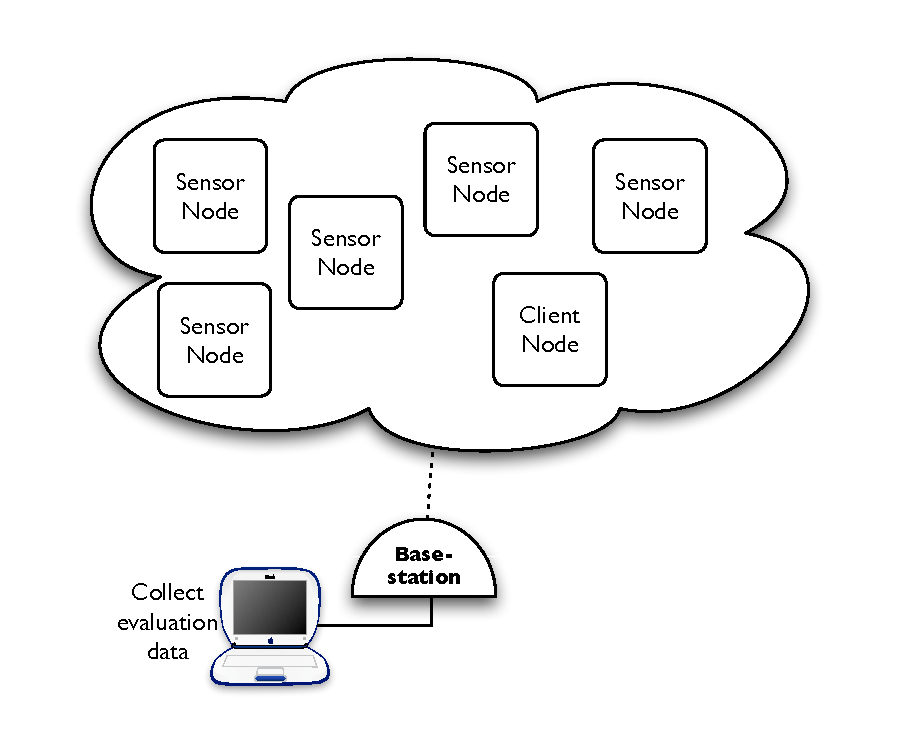
\includegraphics[scale=0.50]{img/EvaluationConfig.eps} 
\caption[Test-bed model of WSN using the DADT/LN prototype]{Test-bed model of WSN using the DADT/LN prototype}
\label{Fig:EvaluationConfig}
\end{figure}

The sensor device that ran the SensorNode application used the temperature and
light sensors available on the Sun SPOT demo sensor board. The DADT/LN prototype
on the sensor device abstracted those sensors using ADT instances, and provided
functionality to perform sensing and resetting operations. Communication between
sensor devices was supported by the LN implementation.

The sensor device that runs the ClientNode application was programmed to 
calculate the average temperature or luminosity value sensed by the set of
nodes. This set of nodes was specified implicitly using a DADT Dataview object
(see Section \ref{subsubsec:views}).


\section{Metrics}

The DADT/LN prototype was evaluated using the following metrics:
\begin{itemize}
\item Memory usage
\item Processing and communication delays
\end{itemize} 

These metrics were selected due to the fact that they allow to  ..  

%Here you need to "define" the various metrics, say what they are and so on...
%More importantly, however, you need to say *why* you picked these metrics and
%why they are important, which you completely miss right now. For instance,
%memory usage is important to measure because it determines how complex your
%application can be while still fitting in the node's memory. Delays are
%important to measure because they determine how scalable is the solution
%w.r.t. the number of DADT properties involved, number of devices in the
%network and so on... For each metric, you also need to say how you measured
%it. For instance, how did you measure the delays? Did you somewhat instrument
%the code?

\section{Results}

\subsection{Memory Usage}

As mentioned above, the memory requirements of the DADT/LN implementation are
based on the following components:
\begin{itemize}
  \item Distributed application code translated and compiled from dadt files
  \item The runtime library of the DADT/LN prototype
\end{itemize}



Table \ref{Tab:Memory} presents the memory requirements for the evaluated sample
distributed application.

\begin{table}

	\begin{center}
	\begin{tabular}{| p{1.8cm} | p{1.8cm} | p{1.8cm} |}
	\hline
	
	%There are free tools online to gather various statistics on source code
	% (WINDOWS), e.g., http://sourcecount.com/
	Filename & DADT Source code, bytes  & Java source code, Num of
	code lines Java bytecode size, bytes \\ \hline 
	
	Sensor.java & -  & tbc  3164 \\ \hline
	SensorNode.dadt \T \B & 477 \T \B & tbc \T \B tbc \\ \hline
	ClientNode.dadt \T \B & 841 \T \B & tbc \T \B tbc \\ \hline
	DSensor.dadt \T \B & 303 \T \B & tbc \T \B tbc \\ \hline
	\end{tabular}
	\end{center}
	\caption{Memory usage}
	\label{Tab:Memory}
\end{table}

As discussed before, the runtime library consists of a number
of Java files that provide the functionality of the DADT/LN prototype. The \emph{jar} file representing the runtime
library for the SUN SPOT device requires 81KB of memory. 

The runtime library was later integrated with the SensorNode application code 
resulting in 95KB jar-file. Similarly, the integrated jar-file of the ClientNode
application requires 99 KB of the memory.

\subsection{Processing and Communication Delays}

This section presents evaluation of the round trip delay time required for
executing a distributed sensing operation on the WSN.  

%%

The processing and communication delays were used to compare the performance of
the DADT/LN prototype upon execution of the distributed operation ``average''
over several such Dataviews. %rewrite%

The Dataview used to define the scope of the given distributed operation would be classified as follows:
\begin{itemize}
\item \emph{low} complexity, which consists of up to 3 DADT properties allowing to define
views, such as ``all active temperature sensors'';
\item \emph{moderate} complexity, which uses from 3 to 10 properties that allows to
create views, such as ``all active temperature
sensors with precision > 1.0 and sensor reading greater than 80'';
\item \emph{high} complexity, which uses up to 20 properties. The number of properties that construct such type of Dataviews was
limited by the length of the radiogram size used for communication between Sun SPOTs.
\end{itemize}

\begin{figure}
\centering
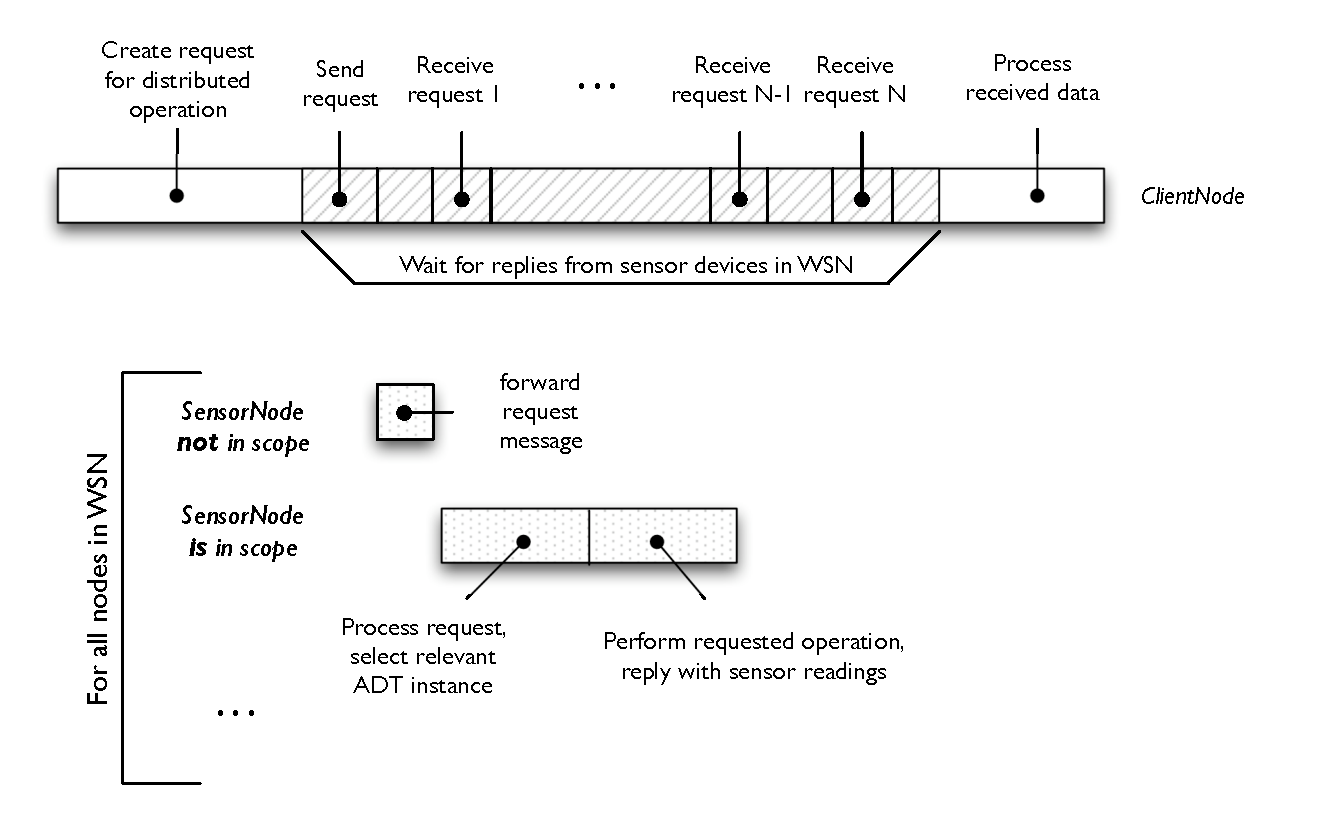
\includegraphics[scale=0.60]{img/RTTevaluation.eps} 
\caption[Delay factors for distributed operation execution]{Factors contributing to delays in the execution of a distributed operation on a WSN using the DADT/LN prototype}
\label{Fig:TimingsModel}
\end{figure}

Figure \ref{Fig:TimingsModel} shows the relevant time delays occurred during the
work of DADT/LN prototype. 

\subsubsection{Non-concurrent requests}

This section provides results of the evaluation of the average time intervals on the basis of single non-concurrent requests.

\begin{table}[h]
\begin{tabular*}{0.85\textwidth}{| p{1.8cm} | p{1.9cm} | p{2.1cm} | p{1.8cm} |
p{1.9cm} | p{1.9cm} | }
\cline{1-6} & \multicolumn{3}{|c|}{ClientNode Application} & \multicolumn{2}{|
c |}{SensorNode Application} \\ \cline{1-6}
Dataview complexity \T \B & Create request (ms) & Send request over LN and wait
for replies (ms) & Process sensor readings (ms) & Receive request, select ADT
instances & Perform requested action and send reply \\ \cline{1-6}
Low & 48.44 & 1154.78 & 220.89 & 251.63 & 86.45  \\ \cline{1-6}
Moderate & 51.36 & 1368.55 & 206.45 & 296.10 & 71.03 \\ \cline{1-6}
High  & 57.67 & 1385.89 & 210.33 & 356.06 & 72.38 \\ \cline{1-6}
\end{tabular*}
\caption{Processing and communication delays for non-concurrent requests for
execution of distributed operation ``average''}
\label{Tab:EvalRes}
\end{table}

As can be seen in Table \ref{Tab:EvalRes}, the complexity of the 
Dataview has a direct correlation to the delays associated with processing of the request
on the SensorNode side. This subsequently leads to increasing waiting
intervals on the ClientNode side.

On the SensorNode, this might be a consequence of the given limitations of the
Squawk JVM, which does not provide support for serialization of objects. Hence,
delays occur when the object representing the scope of the distributed operation is
recreated by the SensorNode, and is later used for identifying the relevant ADT
instances which execute the requested operation.
Activities such as performing an action that involve: (a) requesting sensor
readings, and (b) the subsequent invocation of the LN API to send a reply message, were
executed in a relatively short time.

On the ClientNode, actions such as preparing a request message and parsing
the received results take on average 10-15\% of the time spent waiting for the receipt of reply messages with sensor readings.

\subsubsection{Concurrent requests}

Table \ref{Tab:EvalResConcurrent} shows the processing time delays caused by
concurrent requests on the WSN. The WSN used as part of this evaluation consisted
of two devices running the Client Node application, which issued concurrent
distributed operation execution requests. 
Evaluation of the concurrent requests was based on the assumption that these
requests may be 10-80 ms apart in time.

\begin{table}[h]
\begin{tabular*}{0.85\textwidth}{| p{1.8cm} | p{1.9cm} | p{2.1cm} | p{1.8cm} |
p{1.9cm} | p{1.9cm} | }
\multicolumn{3}{|c|}{ClientNode Application} & \multicolumn{2}{|
c |}{SensorNode Application} \\ \cline{1-6}
Dataview complexity & Create request, ms & Send request over LN and wait
for replies, ms & Process sensor readings, ms & Receive request, select ADT
instances & Perform requested action and send reply \\ \cline{1-6}
High & 64.50 & 1699.80 & 210.00 & 325.23 & 88.06  \\ \cline{1-6}
\end{tabular*}
\caption{Processing and communication delays for concurrent requests for
execution of distributed operation ``average''}
\label{Tab:EvalResConcurrent}
\end{table}

The results presented in Table \ref{Tab:EvalResConcurrent} considered only those
Dataviews with high complexity. 
It can be seen that, in general, concurrent requests increas the processing time
on devices running the SensorNode application only to a little degree. However,
the other delay factors involved in the execution of the distributed operation are comparable to that
incurred upon execution of non-concurrent requests.




